\documentclass{../tuda-beamer}

% Title information
\authors{Simon Hock}
\authors{Nhan Huynh}
\date{10. November 2021}

\begin{document}

  \maketitle

  \begin{frame}{Überblick}
    \tableofcontents
  \end{frame}


  \section{Arrays}
  \begin{frame}{Arrays}
    \begin{itemize}
      \item Block von reserviertem Speicher eines gleichen Komponententyps (Datentyp der Elemente)
      \item Feste Größe
      \item Formaler Aufbau: \inlinejava{Datentyp[] Bezeichner = new Datentyp[Größe];}
      \item Kurzform: \inlinejava{Datentyp[] Bezeichner = \{Element1, Element2, ...\};}
    \end{itemize}
    \begin{figure}[h]
      \centering
      \begin{memory}[scale=.725]
        \allocatedummy{5}
        \allocatedummy{15}
        \allocatedummy{25}
        \allocate{8}{12}
        \allocate{18}{18}
        \assign{23}{18}{\inlinejava{a}}
        \assign{2}{8}{\inlinejava{a[0]}}
        \assign{5}{9}{\inlinejava{a[1]}}
        \assign{8}{10}{\inlinejava{a[2]}}
        \assign{14}{11}{\inlinejava{a[3]}}
        \assign{16}{12}{\inlinejava{a[4]}}
        \assignblock{18}{8}
      \end{memory}
      \caption{Abstrakte Visualisierung des Speicherplatzes eines Arrays \inlinejava{a}}
    \end{figure}
  \end{frame}

  \begin{frame}{Standardwerte}
    \begin{table}[h]
      \rowcolors{2}{white}{gray!25}
      \centering
      \begin{tabular}{ll}
        \toprule
        \textbf{Datentyp} & \textbf{Standardwert}
        \\
        \midrule
        \inlinejava{boolean} & \inlinejava{false}
        \\
        \inlinejava{byte} & \inlinejava{0}
        \\
        \inlinejava{short} & \inlinejava{0}
        \\
        \inlinejava{int} & \inlinejava{0}
        \\
        \inlinejava{long} & \inlinejava{0L}
        \\
        \inlinejava{float} & \inlinejava{0.0f}
        \\
        \inlinejava{double} & \inlinejava{0.0d}
        \\
        \inlinejava{char} & \texttt{\textcolor{stringcolor}{'\textbackslash u0000}'}
        \\
        Referenztypen & \inlinejava{null}
        \\
        \bottomrule
      \end{tabular}
      \caption{Standardwerte für Attribute und Arraykomponenten}
    \end{table}
  \end{frame}

  \begin{frame}{Analogie - Bücherregal}
    \begin{itemize}
      \item Vorstellung Array als Bücherregal
      \item Größe des Arrays: Anzahl an Fächern
      \item Fach kann nur ein Buch aufbewahren (eindimensionales Array)
    \end{itemize}
    \begin{figure}[h]
      \centering
      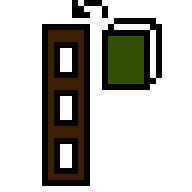
\includegraphics[width=.2\linewidth]{graphics/lib_1_1.png}
      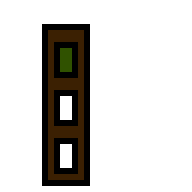
\includegraphics[width=.2\linewidth]{graphics/lib_1_2.png}
      \caption{Array als Bücherregal}
    \end{figure}
  \end{frame}

  \begin{frame}[c]
    \begin{figure}[h]
      \centering
      \lstinputlisting[style=Java, title=Klasse Book]{codes/Book.java}
    \end{figure}
  \end{frame}

  \begin{frame}[c]
    \lstinputlisting[style=Java, title=Bücherregal als Array]{codes/Book_Array.java}
  \end{frame}

  \begin{frame}
    \lstinputlisting[
      style=Java,
      title=Bücherregal als Array - Kurzform]
    {codes/Book_Array_Shortform.java}
  \end{frame}

  \begin{frame}[c]
    \begin{figure}[h]
      \centering
      
\includegraphics[width=.2\linewidth]{graphics/lib_2_1.png}
      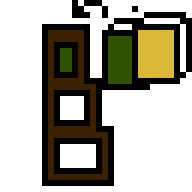
\includegraphics[width=.2\linewidth]{graphics/lib_2_2.png}
      
\includegraphics[width=.2\linewidth]{graphics/lib_2_3.png}
      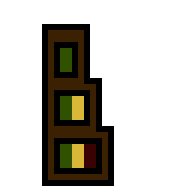
\includegraphics[width=.2\linewidth]{graphics/lib_2_4.png}
      \caption{Verschachteltes Array als Bücherregal}
    \end{figure}
  \end{frame}

  \begin{frame}[c]
    \begin{figure}[h]
      \centering
      \lstinputlisting[
        style=Java, lastline=9,
        title=Bücherregal als verschachteltes Array]
      {codes/Book_Array_Nested.java}
    \end{figure}
  \end{frame}

  \begin{frame}[c]
    \begin{figure}[h]
      \centering
      \lstinputlisting[
        style=Java, firstline=12,
        firstnumber=11,
        title=Bücherregal als verschachteltes Array]
      {codes/Book_Array_Nested.java}
    \end{figure}
  \end{frame}


  \section{JUnit}
  \begin{frame}{JUnit - Testen}
    \begin{itemize}
      \item Framework zum Testen von Java-Programmen
      \item JUnit 5
      \item Testen von Methoden auf Korrektheit
      \item Später Vorführung
    \end{itemize}
  \end{frame}

  \begin{frame}{JUnit - Importe}
    \begin{itemize}
      \item \inlinejava{org.junit.Assert}/ \inlinejava{org.junit.api.Assertions}
      \begin{itemize}
        \item Sammlung von Klassenmethoden zum Testen.
        \item \inlinejava{Assert}: Existiert nur noch aus Kompatibilitätsgründen.
        \item \inlinejava{Assertions}: Enthält die neueren JUnit 5 Funktionalitäten.
        \begin{itemize}
          \item \url{https://junit.org/junit5/docs/5.0.1/api/org/junit/jupiter/api/Assertions.html}
        \end{itemize}
      \end{itemize}
      \item \inlinejava{org.junit.jupiter.api}
      \begin{itemize}
        \item Wichtige Funktionalitäten zum Testen bspw. \inlinejava{@Test} Annotation.
      \end{itemize}
    \end{itemize}
  \end{frame}

  \begin{frame}{JUnit-Annotationen}
    \begin{table}[h]
      \rowcolors{2}{white}{gray!25}
      \centering
      \begin{tabular}{lp{12cm}}
        \toprule
        \textbf{Annotation} & \textbf{Beschreibung}
        \\
        \midrule
        \inlinejava{@Test} & Annotierte Methode ist eine Testmethode.
        \\
        \inlinejava{@BeforeAll} & Annotierte Methode wird vor allen Tests in der aktuellen
        Testklasse ausgeführt.
        \\
        \inlinejava{@AfterAll} & Annotierte Methode wird nach allen Tests in der aktuellen
        Testklasse ausgeführt.
        \\
        \inlinejava{@BeforeEach} & Annotierte Methode wird vor jeden Test in der aktuellen
        Testklasse ausgeführt
        \\
        \inlinejava{@AfterEach} & Annotierte Methode ist eine Testmethode.
        \\
        \bottomrule
      \end{tabular}
      \caption{Wichtige Annotationen}
    \end{table}
  \end{frame}

  \begin{frame}
    \begin{figure}[h]
      \centering
      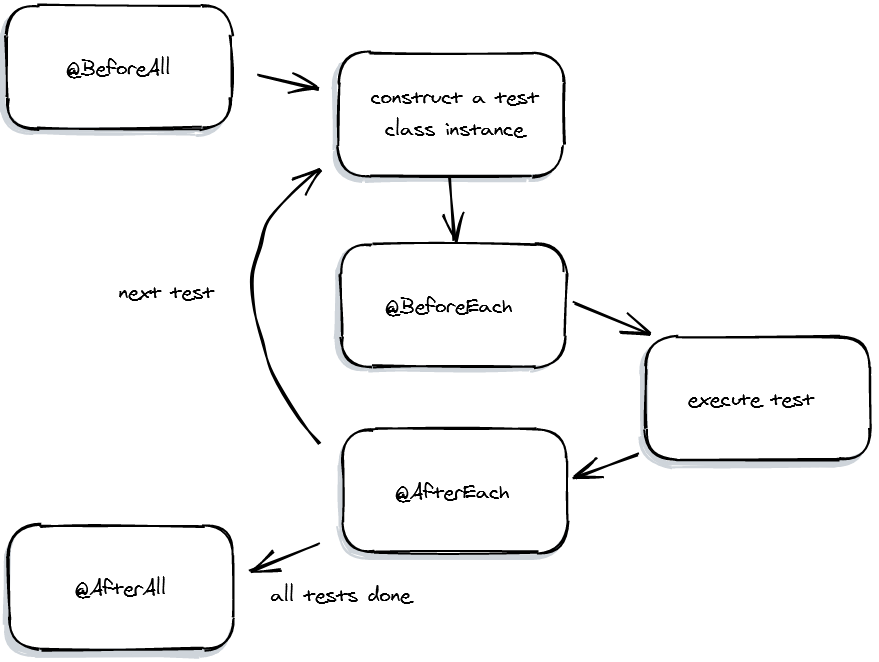
\includegraphics[width=.525\linewidth]{graphics/junit_annotations_order_execution.png}
      \caption{Quelle: \url{https://www.arhohuttunen.com/junit-5-test-lifecycle/}}
    \end{figure}
  \end{frame}

  \begin{frame}[c]
    \begin{center}
      \textbf{\LARGE Live Coding}
    \end{center}
  \end{frame}


  \section{Arbeitsphase}
  \begin{frame}[c]{Arbeitsphase}
    \begin{center}
      \textbf{\LARGE Selbstständiges Arbeiten}
    \end{center}
  \end{frame}
\end{document}
